\documentclass[handout]{beamer}
\usepackage{tikz}
\def\checkmark{\tikz\fill[scale=0.4](0,.35) -- (.25,0) -- (1,.7) -- (.25,.15) -- cycle;} 
\usepackage{pifont}
\newcommand{\xmark}{\ding{55}}
\usepackage{animate}
\usepackage{xcolor,cancel}

\usetheme{PaloAlto}
\title{Practical ODE modelling}
\author[Ben]{Ben Lambert$^1$}
\usepackage{datetime}
\newdate{date}{8}{2}{2021}
\date{\displaydate{date}}
\institute[University of Oxford]{
	\inst{1}University of Oxford}
\beamertemplatenavigationsymbolsempty
\setbeamertemplate{sidebar left}{}

\makeatletter
\newcommand\mathcircled[1]{%
	\mathpalette\@mathcircled{#1}%
}
\newcommand\@mathcircled[2]{%
	\tikz[baseline=(math.base)] \node[draw,circle,inner sep=1pt] (math) {$\m@th#1#2$};%
}

\begin{document}

\begin{frame}
\titlepage
\end{frame}

\begin{frame}
	\frametitle{Lecture outcomes}
	
	\begin{enumerate}
		\item Explain difficulty with inference for ODEs;
		\item Inference with PINTS and other libraries;
		\item PINTS demo.
	\end{enumerate}
	
\end{frame}

\section{ODE inference refresh}
\frame{\tableofcontents[currentsection]}

\begin{frame}
	\frametitle{Setting up the inference problem: forward model}

	
	\begin{equation}
	\frac{d y(t)}{dt} = f(y, t; \theta).
	\end{equation}
	
	\begin{figure}
		\centerline{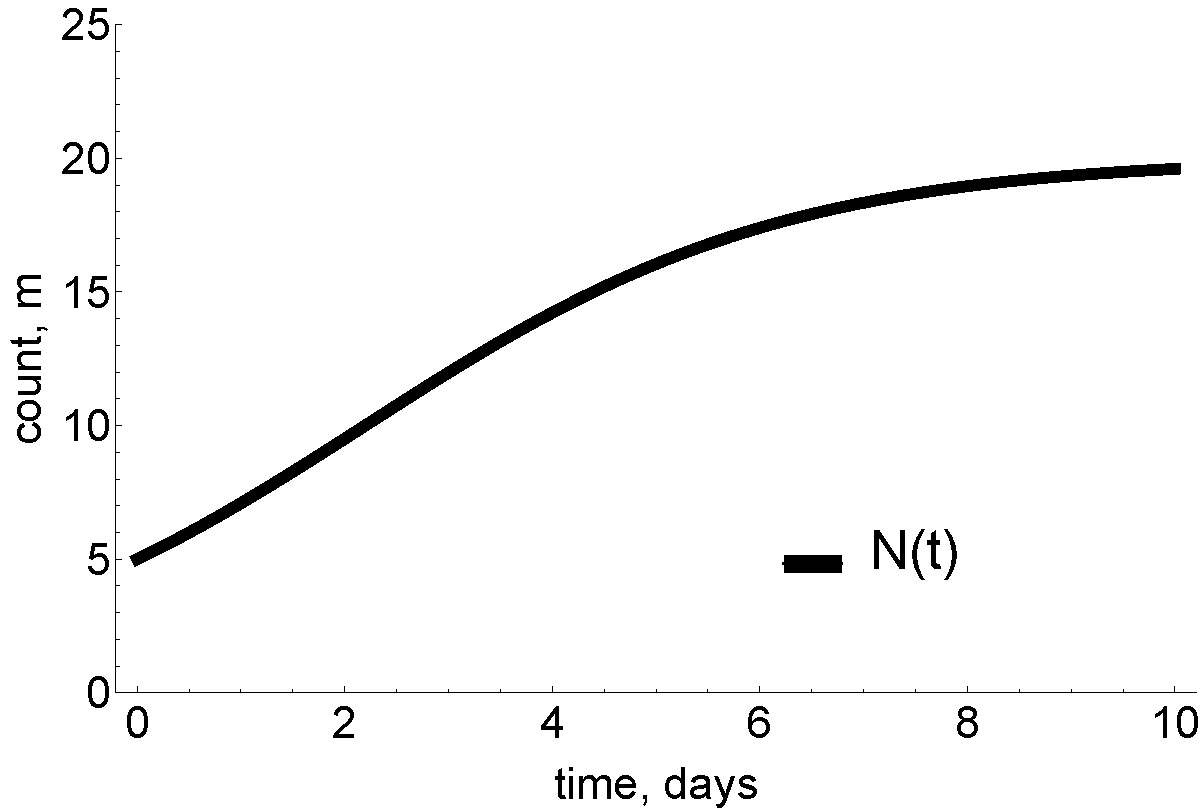
\includegraphics[width=0.7\textwidth]{./Figures/lec7_odeSingleBulding1.pdf}}
	\end{figure}
	
\end{frame}

\begin{frame}
	\frametitle{Setting up the inference problem: noise model}
	
	
	\begin{equation}
	y^*(t) \stackrel{i.i.d.}{\sim} \mathcal{N}(y(t;\theta), \sigma).
	\end{equation}
	
	\begin{figure}
		\centerline{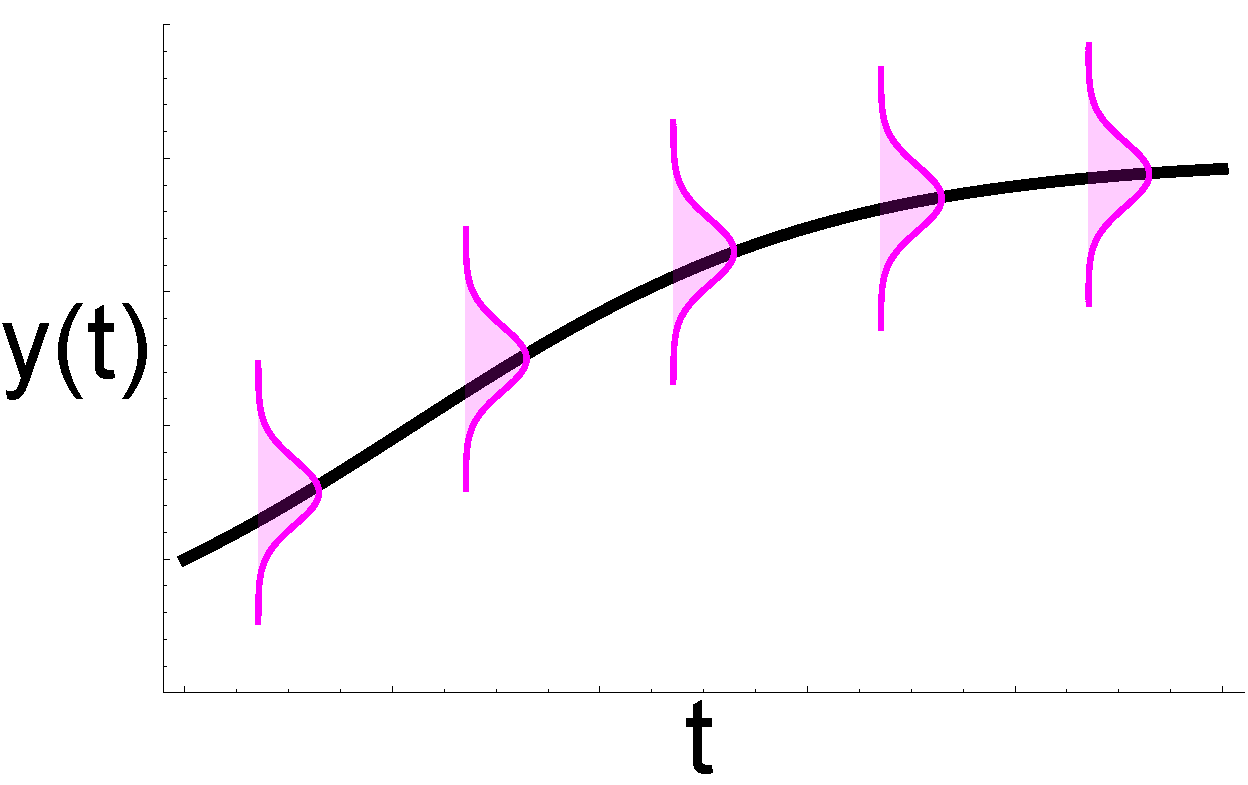
\includegraphics[width=0.7\textwidth]{./Figures/lec7_odeSingleBulding2.pdf}}
	\end{figure}
	
\end{frame}

\begin{frame}
	\frametitle{Setting up the inference problem: data}
	
	\begin{equation}
	\mathcal{L} = \prod_{i=1}^{S} \mathcal{N}(y^*(t_i)| y(t_i;\theta), \sigma).
	\end{equation}
	
	\begin{figure}
		\centerline{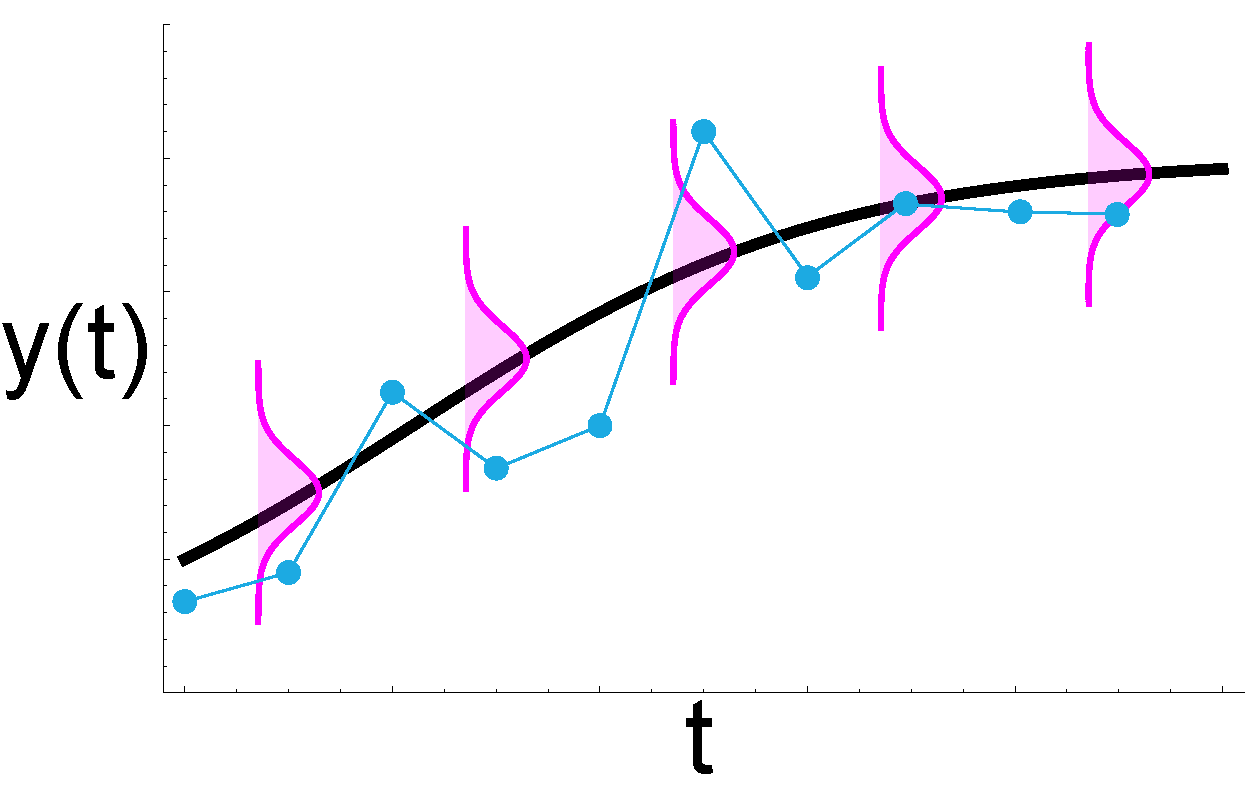
\includegraphics[width=0.7\textwidth]{./Figures/lec7_odeSingleBulding2_data.pdf}}
	\end{figure}
	
\end{frame}

\begin{frame}
	\frametitle{Setting up the inference problem: posterior}
	
	\begin{equation}
	p(\theta|X) \propto p(\theta,\sigma) \prod_{i=1}^{S} \mathcal{N}(y^*(t_i)| y(t_i;\theta), \sigma).
	\end{equation}
	
	\begin{figure}
		\centerline{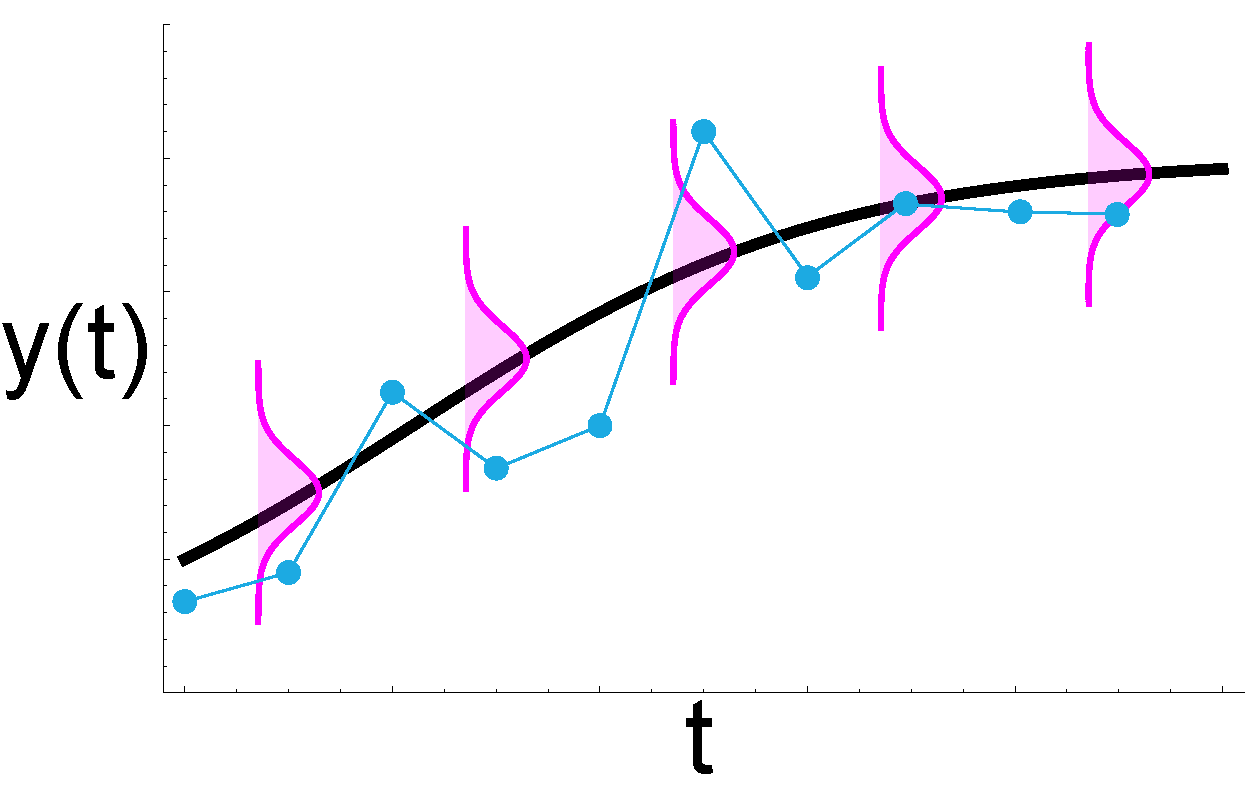
\includegraphics[width=0.7\textwidth]{./Figures/lec7_odeSingleBulding2_data.pdf}}
	\end{figure}
	
\end{frame}

\section{Issues with ODE inference}
\frame{\tableofcontents[currentsection]}

\begin{frame}
	\frametitle{Why is inference for ODEs hard?}
	
	\begin{itemize}
		\item ODEs (typically) require numerical solutions $\implies$ expensive;
		\item Non-linearity $\implies$ posterior distributions can be complex / unidentified.
	\end{itemize}
	
\end{frame}

\begin{frame}
	\frametitle{Why is inference for ODEs hard?}
	
	\begin{figure}
		\centerline{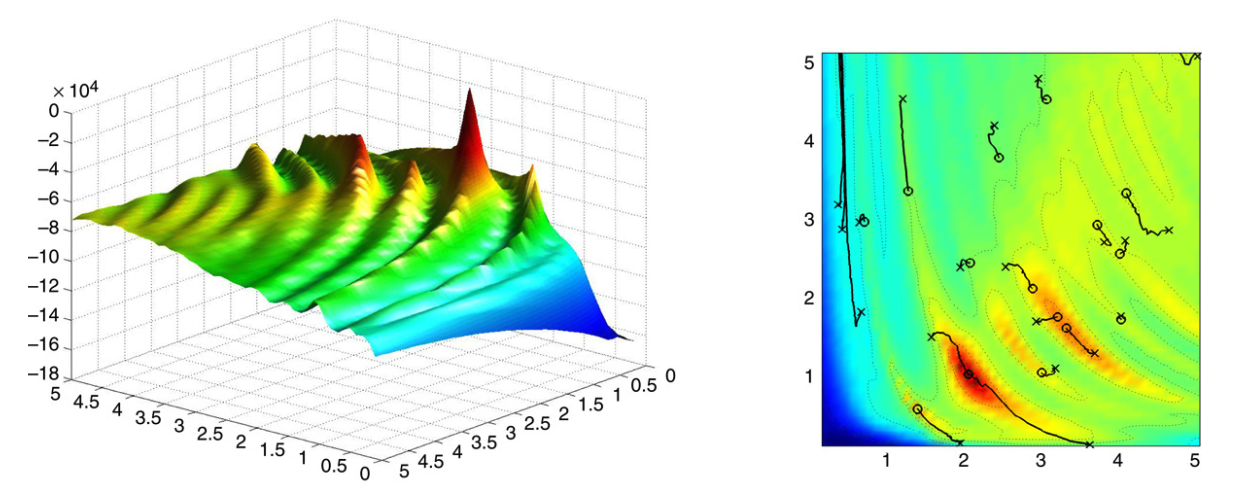
\includegraphics[width=1\textwidth]{./Figures/girolami.png}}
	\end{figure}
	
	from ``Bayesian inference for differential equations'', Girolami (2008)
	
	
\end{frame}

\begin{frame}
	\frametitle{How to make your life easier}
	
	Before you start inference:
	
	\begin{itemize}
		\item Fake data simulation followed by inference: make simulated data as similar to real data characteristics as possible;
		\item Profile likelihood method to assess identifiability;
		\item General mathematical analysis: assess sensitivity of outputs to parameters.
	\end{itemize}
\end{frame}

\section{Inference cycle}
\frame{\tableofcontents[currentsection]}

\begin{frame}
	\frametitle{How to fit model to data?}
	
	\begin{figure}
		\centerline{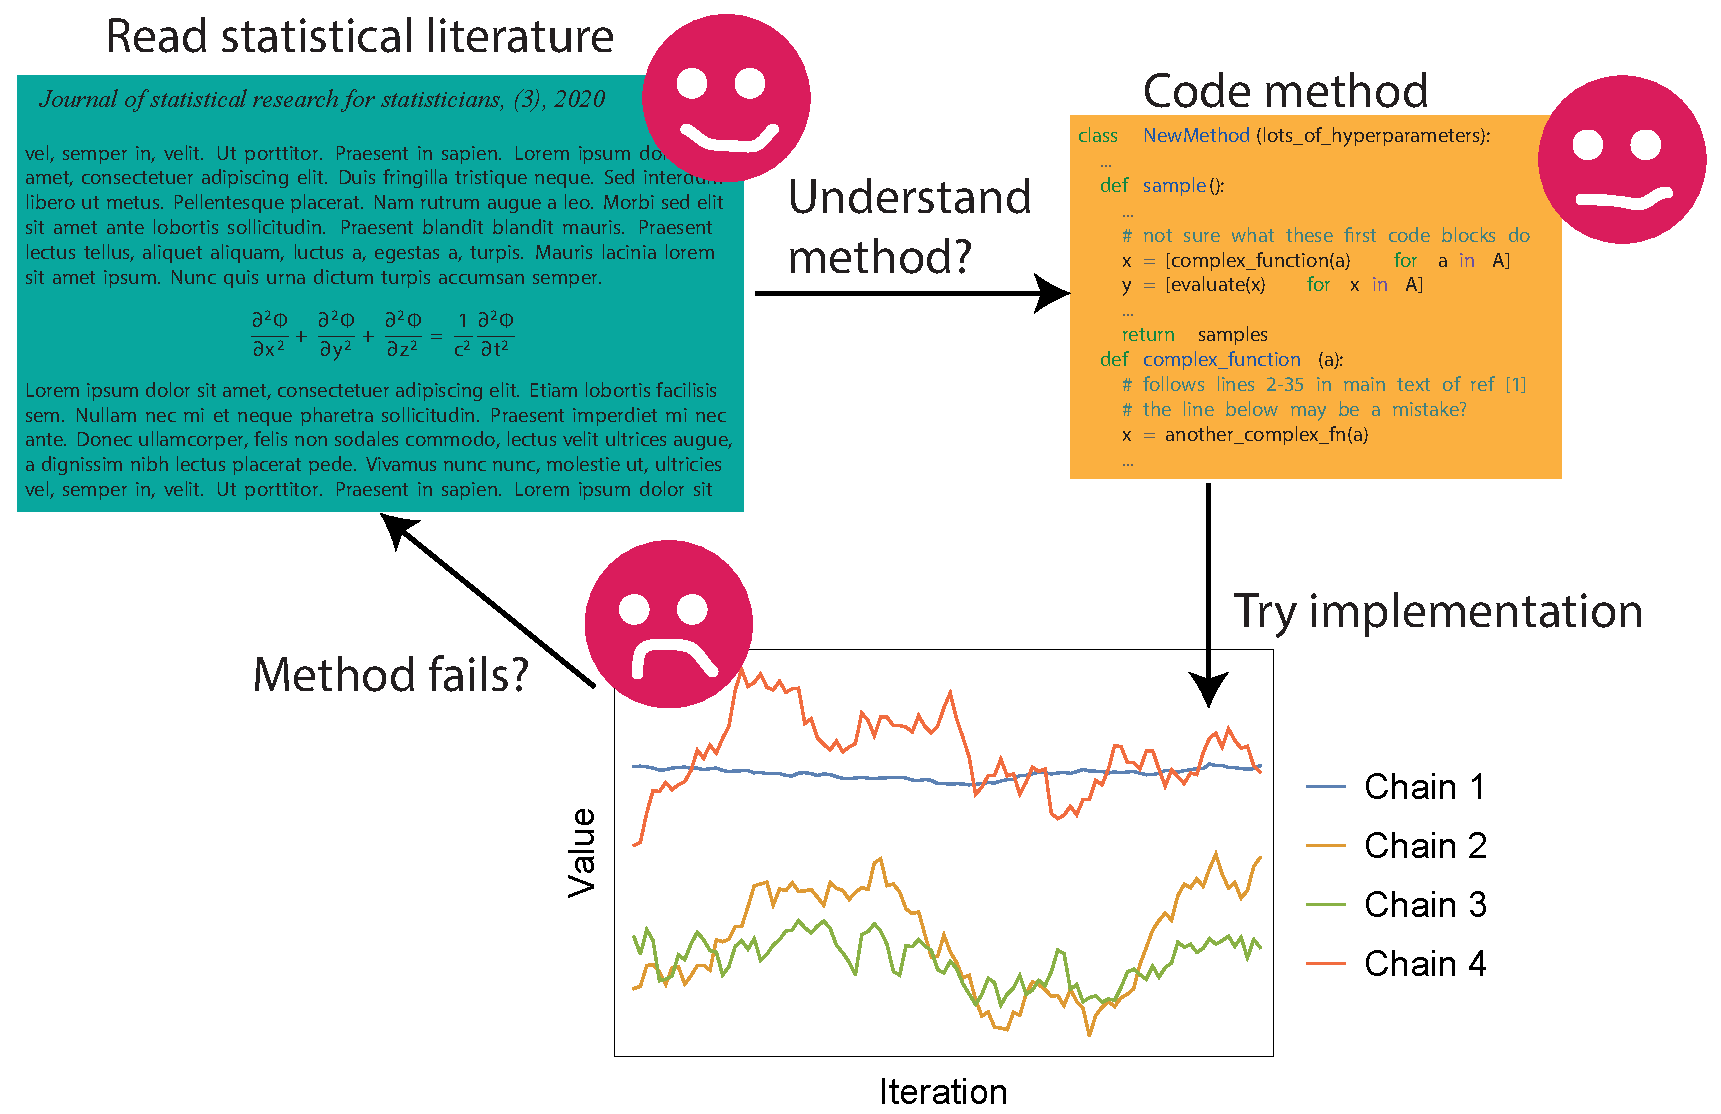
\includegraphics[width=1\textwidth]{./Figures/student_cycle.pdf}}
	\end{figure}
	
\end{frame}

\begin{frame}
	\frametitle{Why does this cycle of misery persist?}
	
	\begin{itemize}
		\item Statistical literature is written by methods experts for other experts;
		\item Statistics papers do not often contain high quality pseudocode;
		\item Software accompanying papers is typically not professionally developed;
		\item Software is typically idiosyncratic;
		\item Different problems require different solutions but solutions currently require reinventing the wheel;
		\item Not enough knowledge sharing between applied researchers about ``Which method works best?''.
	\end{itemize}
	
\end{frame}

\begin{frame}
\frametitle{What is PINTS?}

PINTS: \textbf{P}robabilistic \textbf{I}nference for \textbf{N}oisy \textbf{T}ime \textbf{S}eries, which covers two broad categories of inference methods:

\begin{itemize}
	\item Optimisation: single set of parameters returned;
	\item Sampling: many sets returned.
\end{itemize}

It's an open-source Python library available on Github.

\end{frame}


\begin{frame}
\frametitle{What does existing literature do?}


\begin{itemize}
	\item Most other inference software pin their hope on a single sampler:
	\begin{itemize}
		\item BUGS and JAGS: Gibbs sampler;
		\item PyMC3 and Stan: No U-Turn Sampler (NUTS);
	\end{itemize}
	\item Other libraries prepackage forward model solution methods with sampling method.
\end{itemize}

\end{frame}

\begin{frame}
	\frametitle{How is PINTS different?}
	\begin{itemize}
		\item PINTS not aligned to a single algorithm;
		\item PINTS is designed to interface with (other) probabilistic programming languages (for example, Stan);
		\item PINTS aimed at harder forward models: ODEs and PDEs;
		\item PINTS allows users freedom to use own forward model solution method.
	\end{itemize}
\end{frame}

\begin{frame}
	\frametitle{PINTS niche}
	
	\begin{figure}
		\centerline{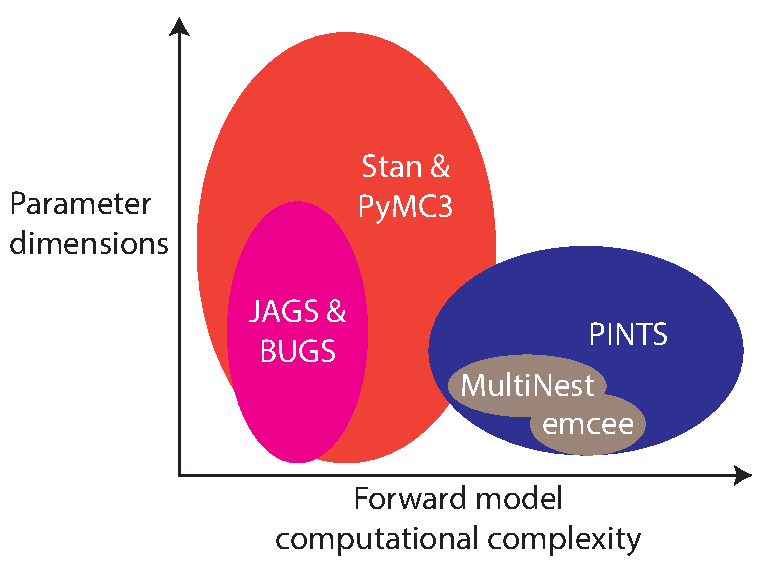
\includegraphics[width=1\textwidth]{./Figures/niche-samplers.pdf}}
	\end{figure}
	
\end{frame}

\begin{frame}
	\frametitle{Deciding on an approach}
	
	\begin{itemize}
		\item For cheap forward model $\implies$ use Stan (you can always use PINTS' Stan interface if this doesn't work);
		\item For expensive forward models, potentially requiring bespoke solvers $\implies$ use PINTS.
	\end{itemize}
	
\end{frame}

\begin{frame}
\frametitle{PINTS in detail}

\begin{itemize}
	\item Literature emphasis on developing new algorithms;
	\item Literature dense with hard-to-decipher algorithm details;
	\item PINTS aims to make this research \textbf{useful}:
	\begin{itemize}
		\item Common, easy-to-use, interface for lots of methods;
		\item Rigorous software development practices;
		\item Many levels of testing: unit, functional, and so on;
		\item Collaboration with statisticians working on various methods;
		\item Benchmark problems;
		\item Pseudocode and tutorial papers which explain algorithms and their ecosystem.
	\end{itemize} 
\end{itemize}

\end{frame}

\begin{frame}
\frametitle{PINTS roadmap: samplers}

\begin{figure}
	\centerline{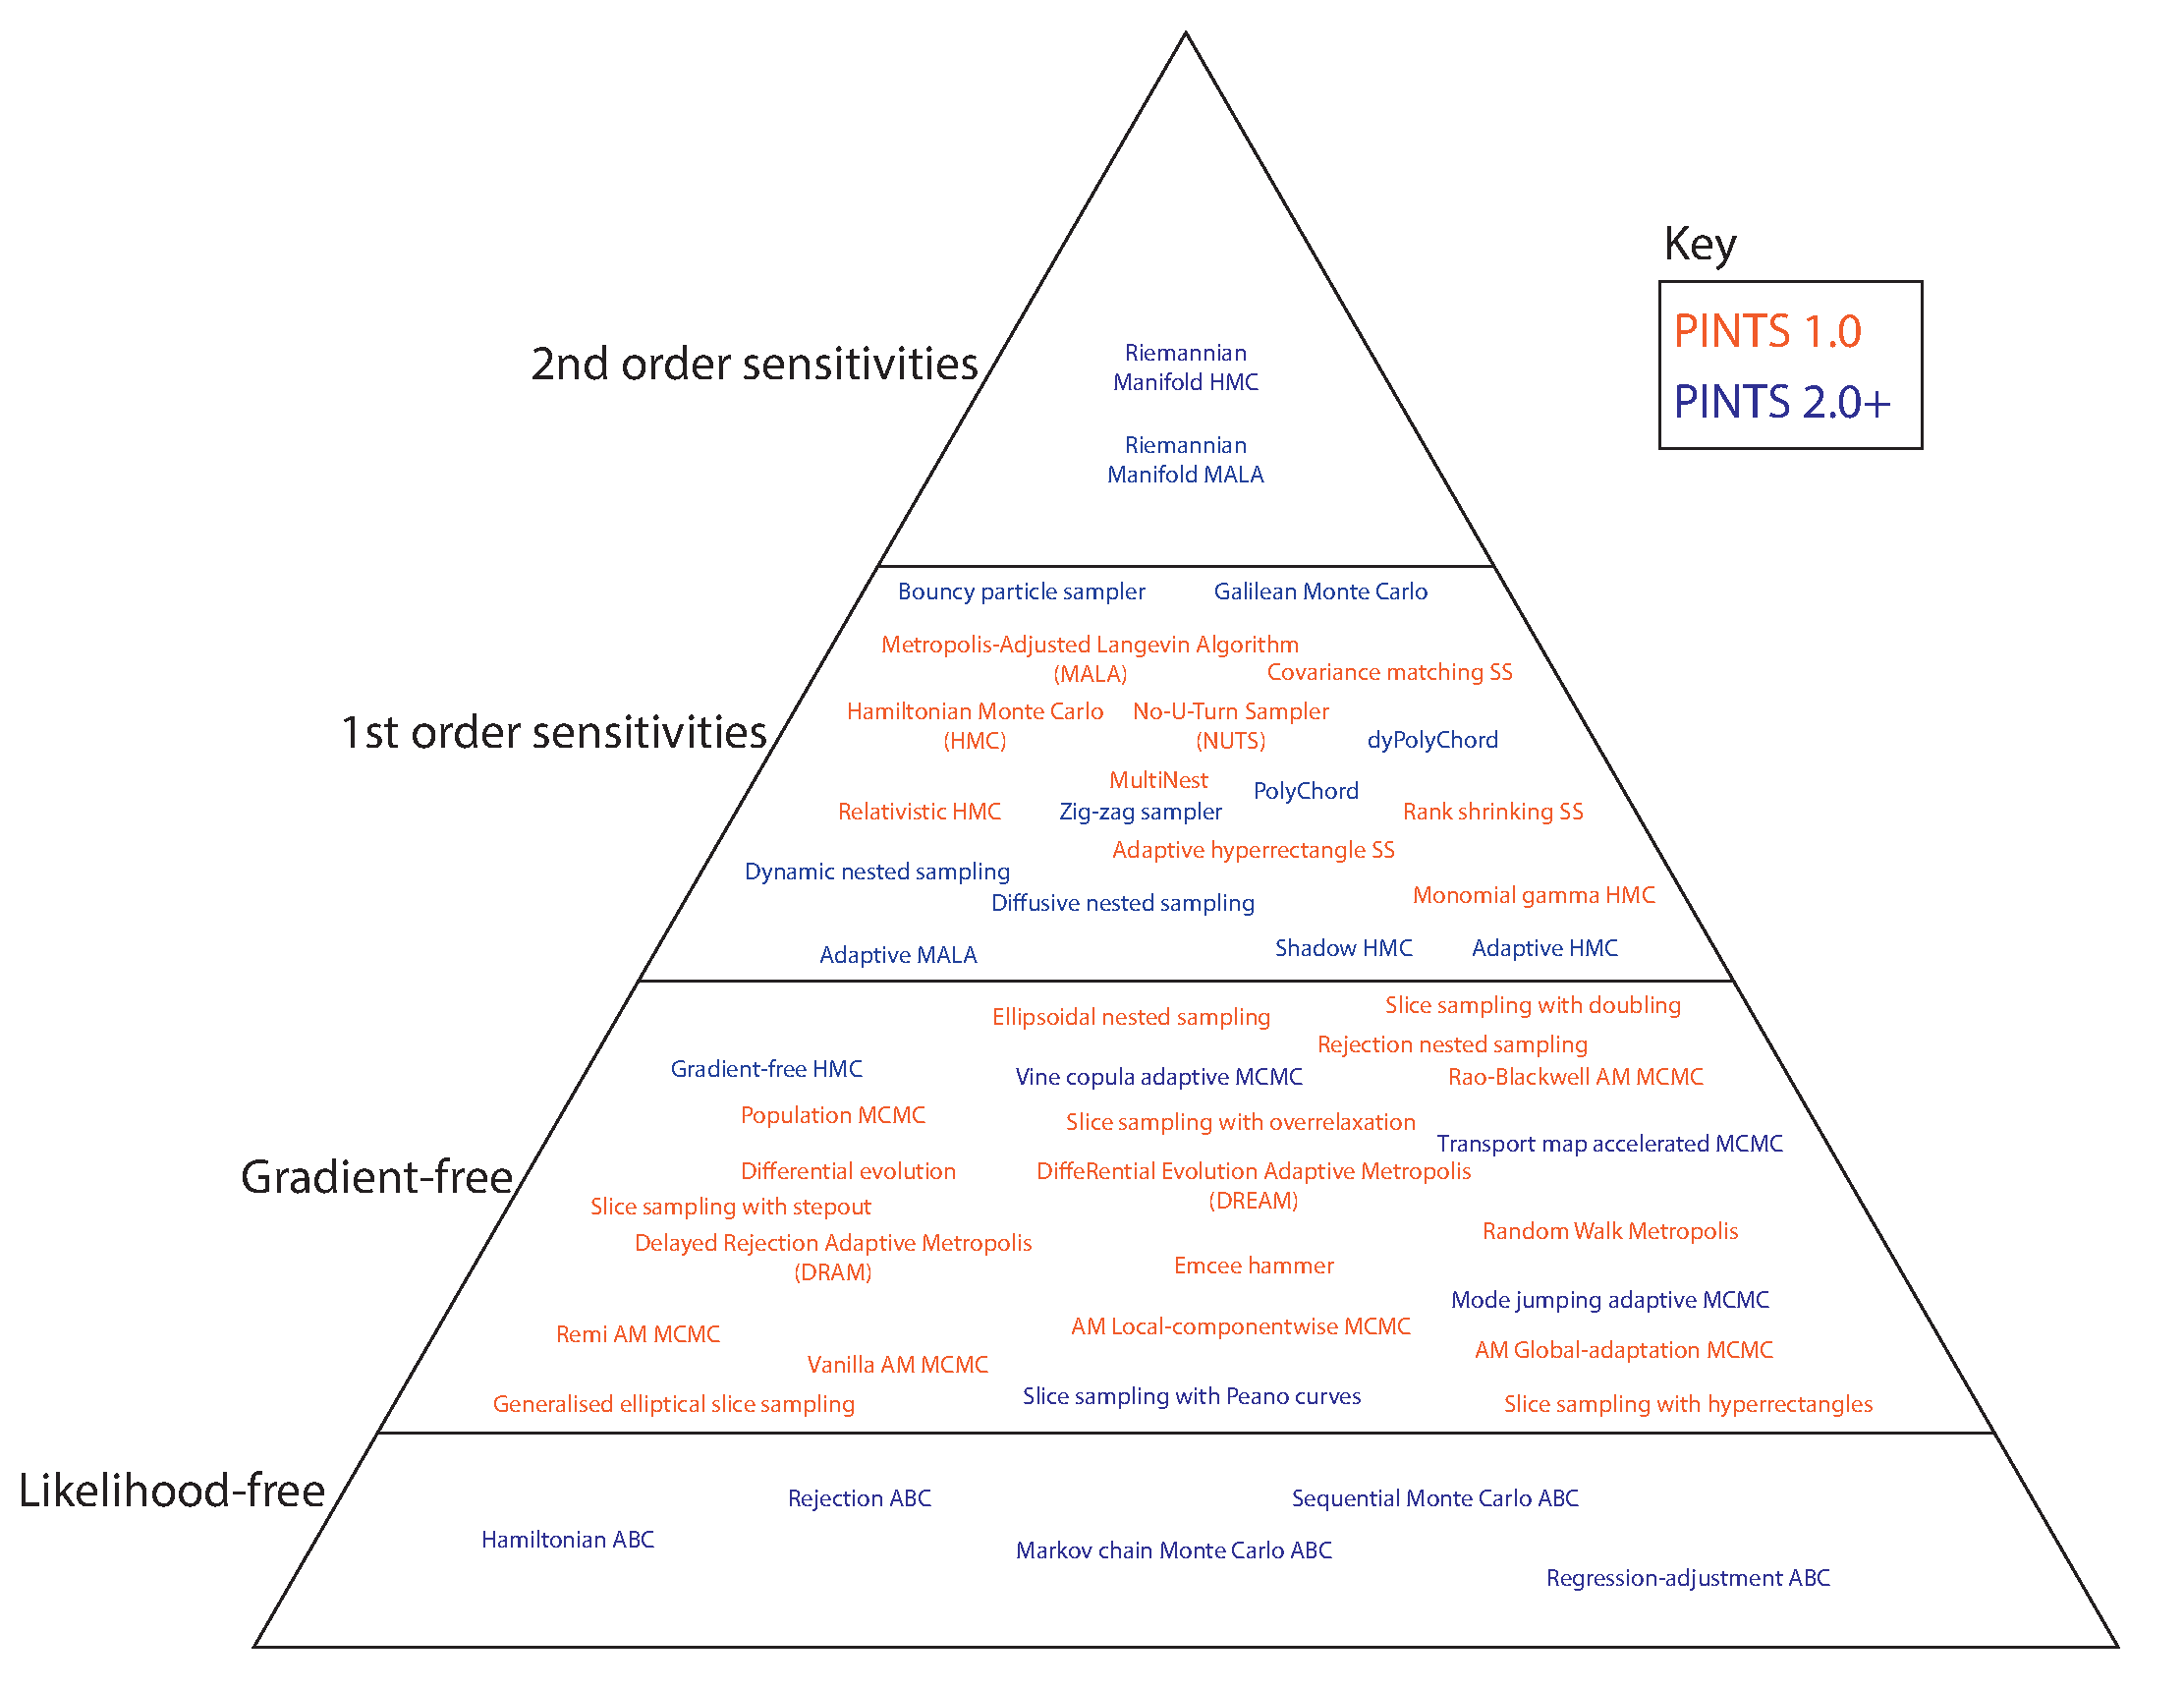
\includegraphics[width=0.9\textwidth]{./Figures/pints-roadmap-triangle-more-samplers.pdf}}
\end{figure}

\end{frame}

\begin{frame}
	\frametitle{Families of samplers: overall}
	
	\begin{figure}
		\centerline{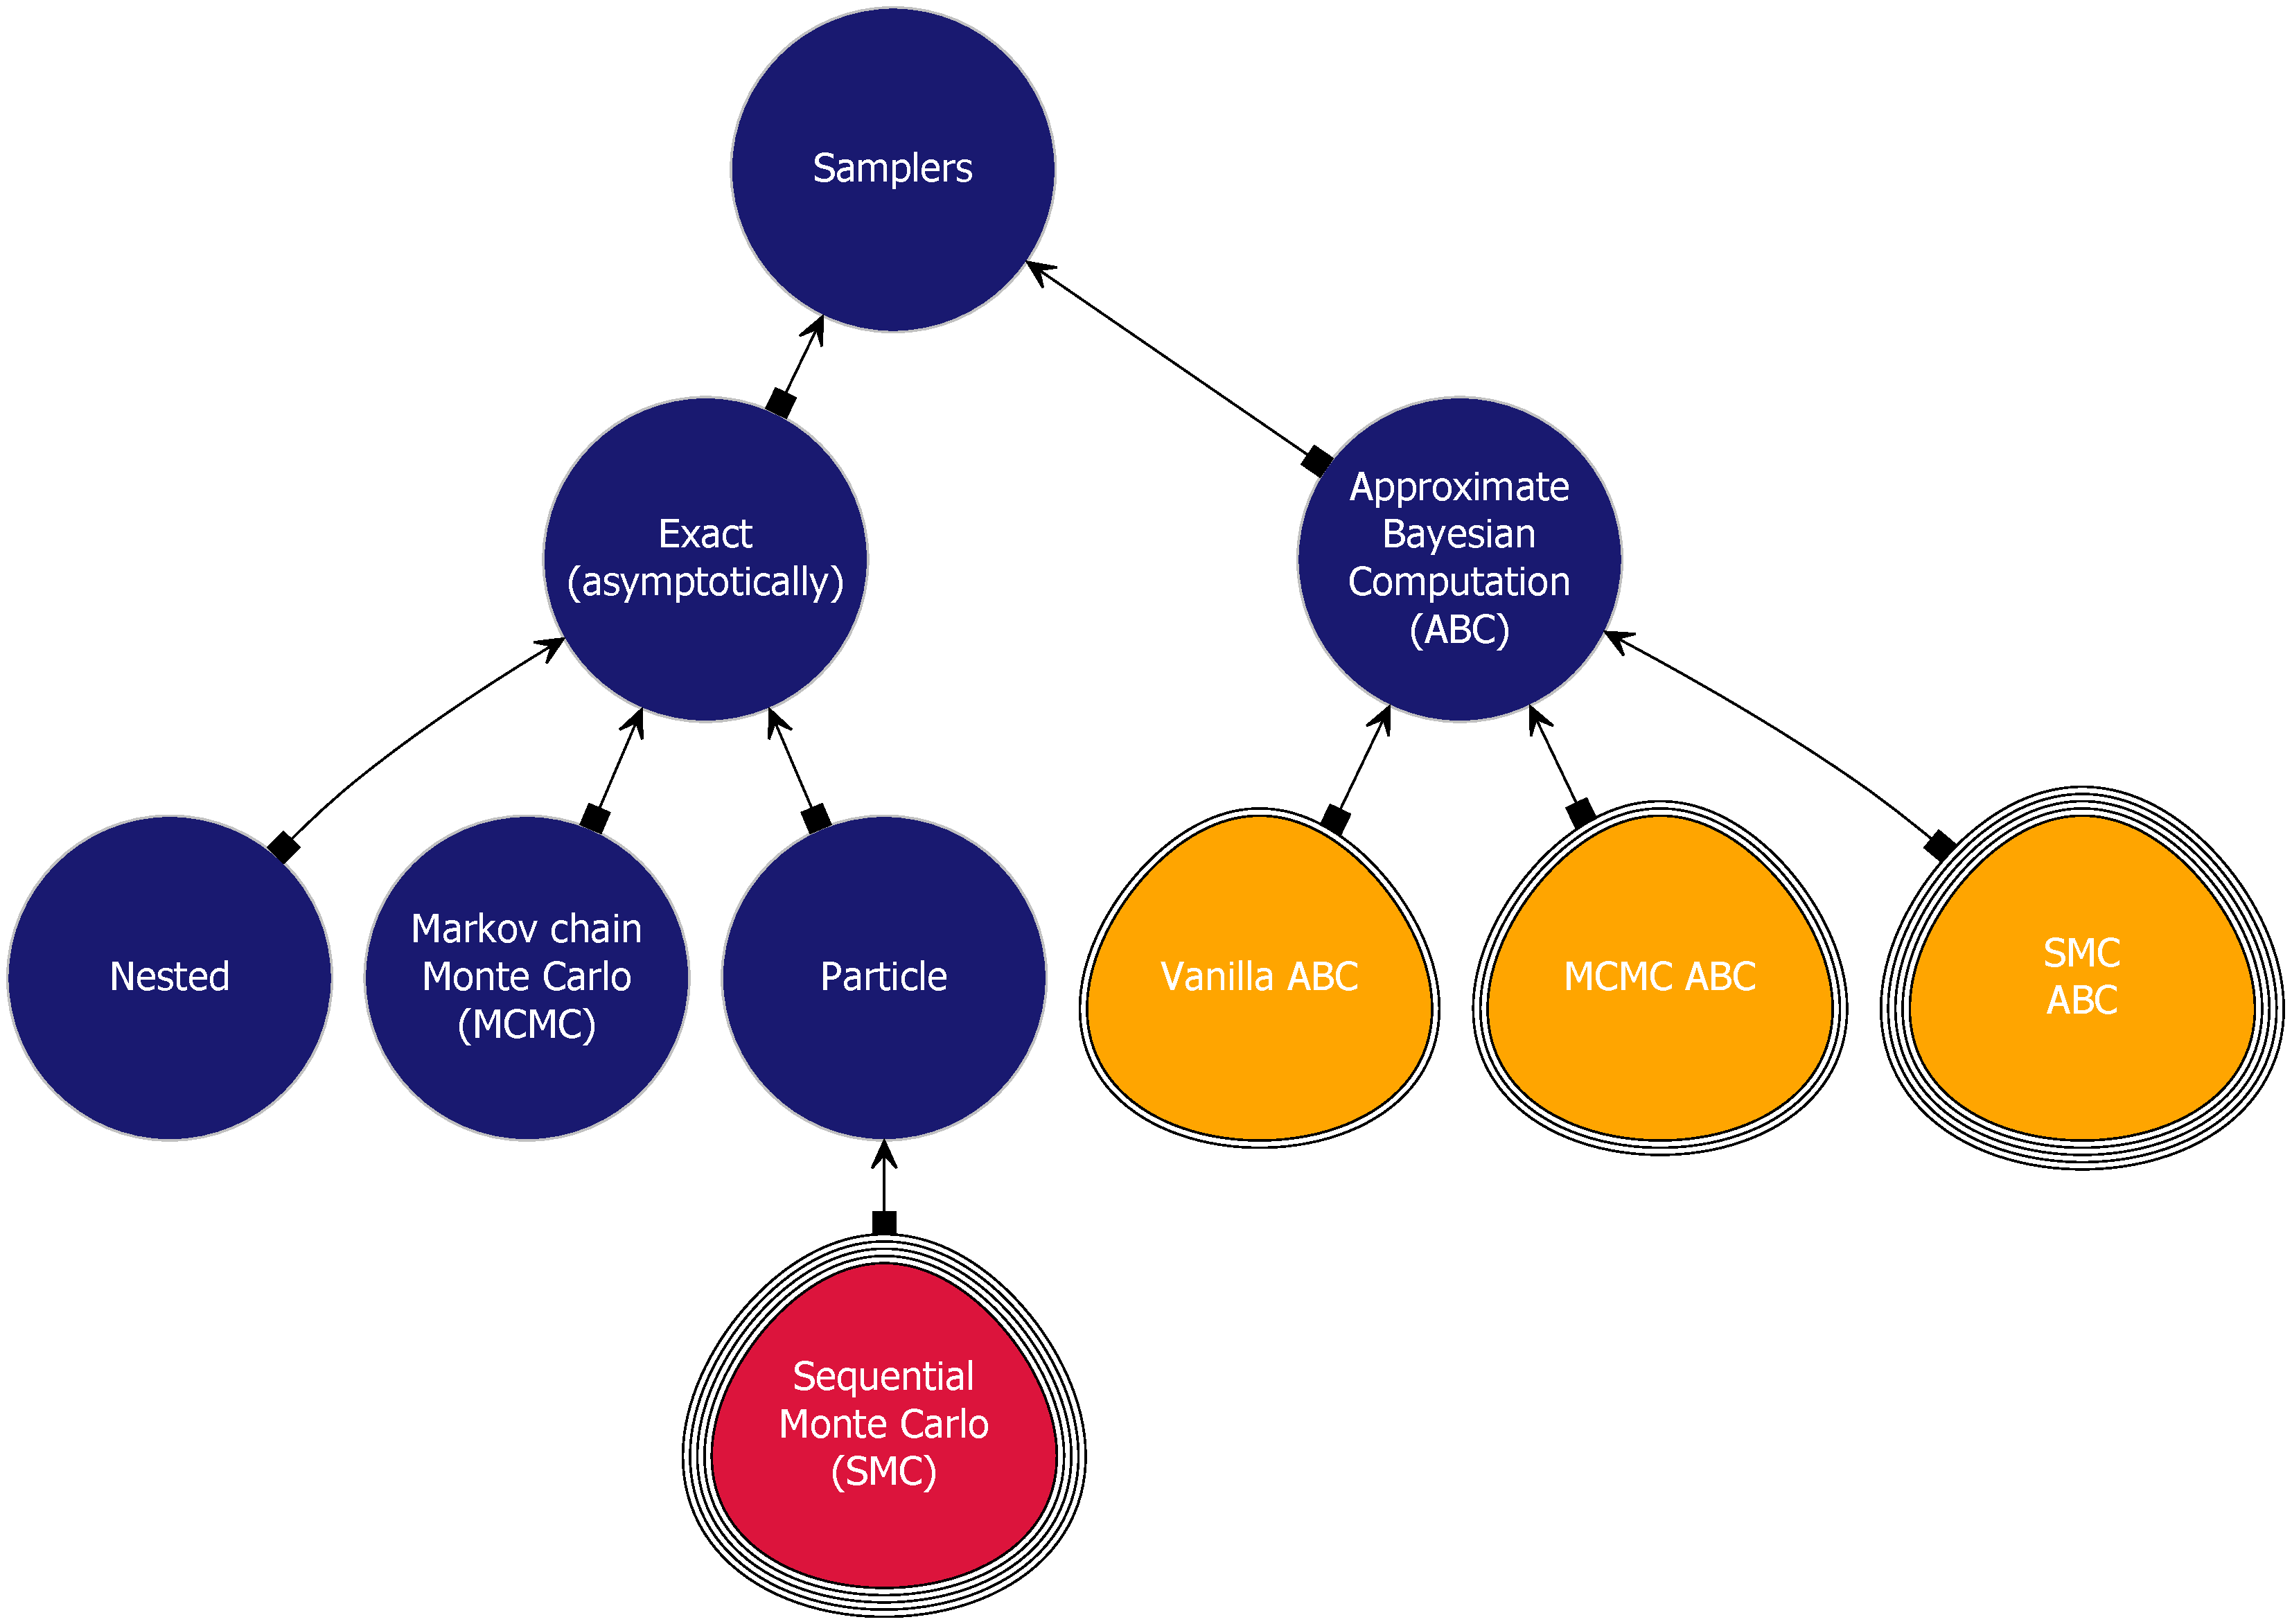
\includegraphics[width=1\textwidth]{./Figures/hierarchy-samplers-top.pdf}}
	\end{figure}
	
\end{frame}

\begin{frame}
	\frametitle{Families of samplers: within MCMC}
	
	\begin{figure}
		\centerline{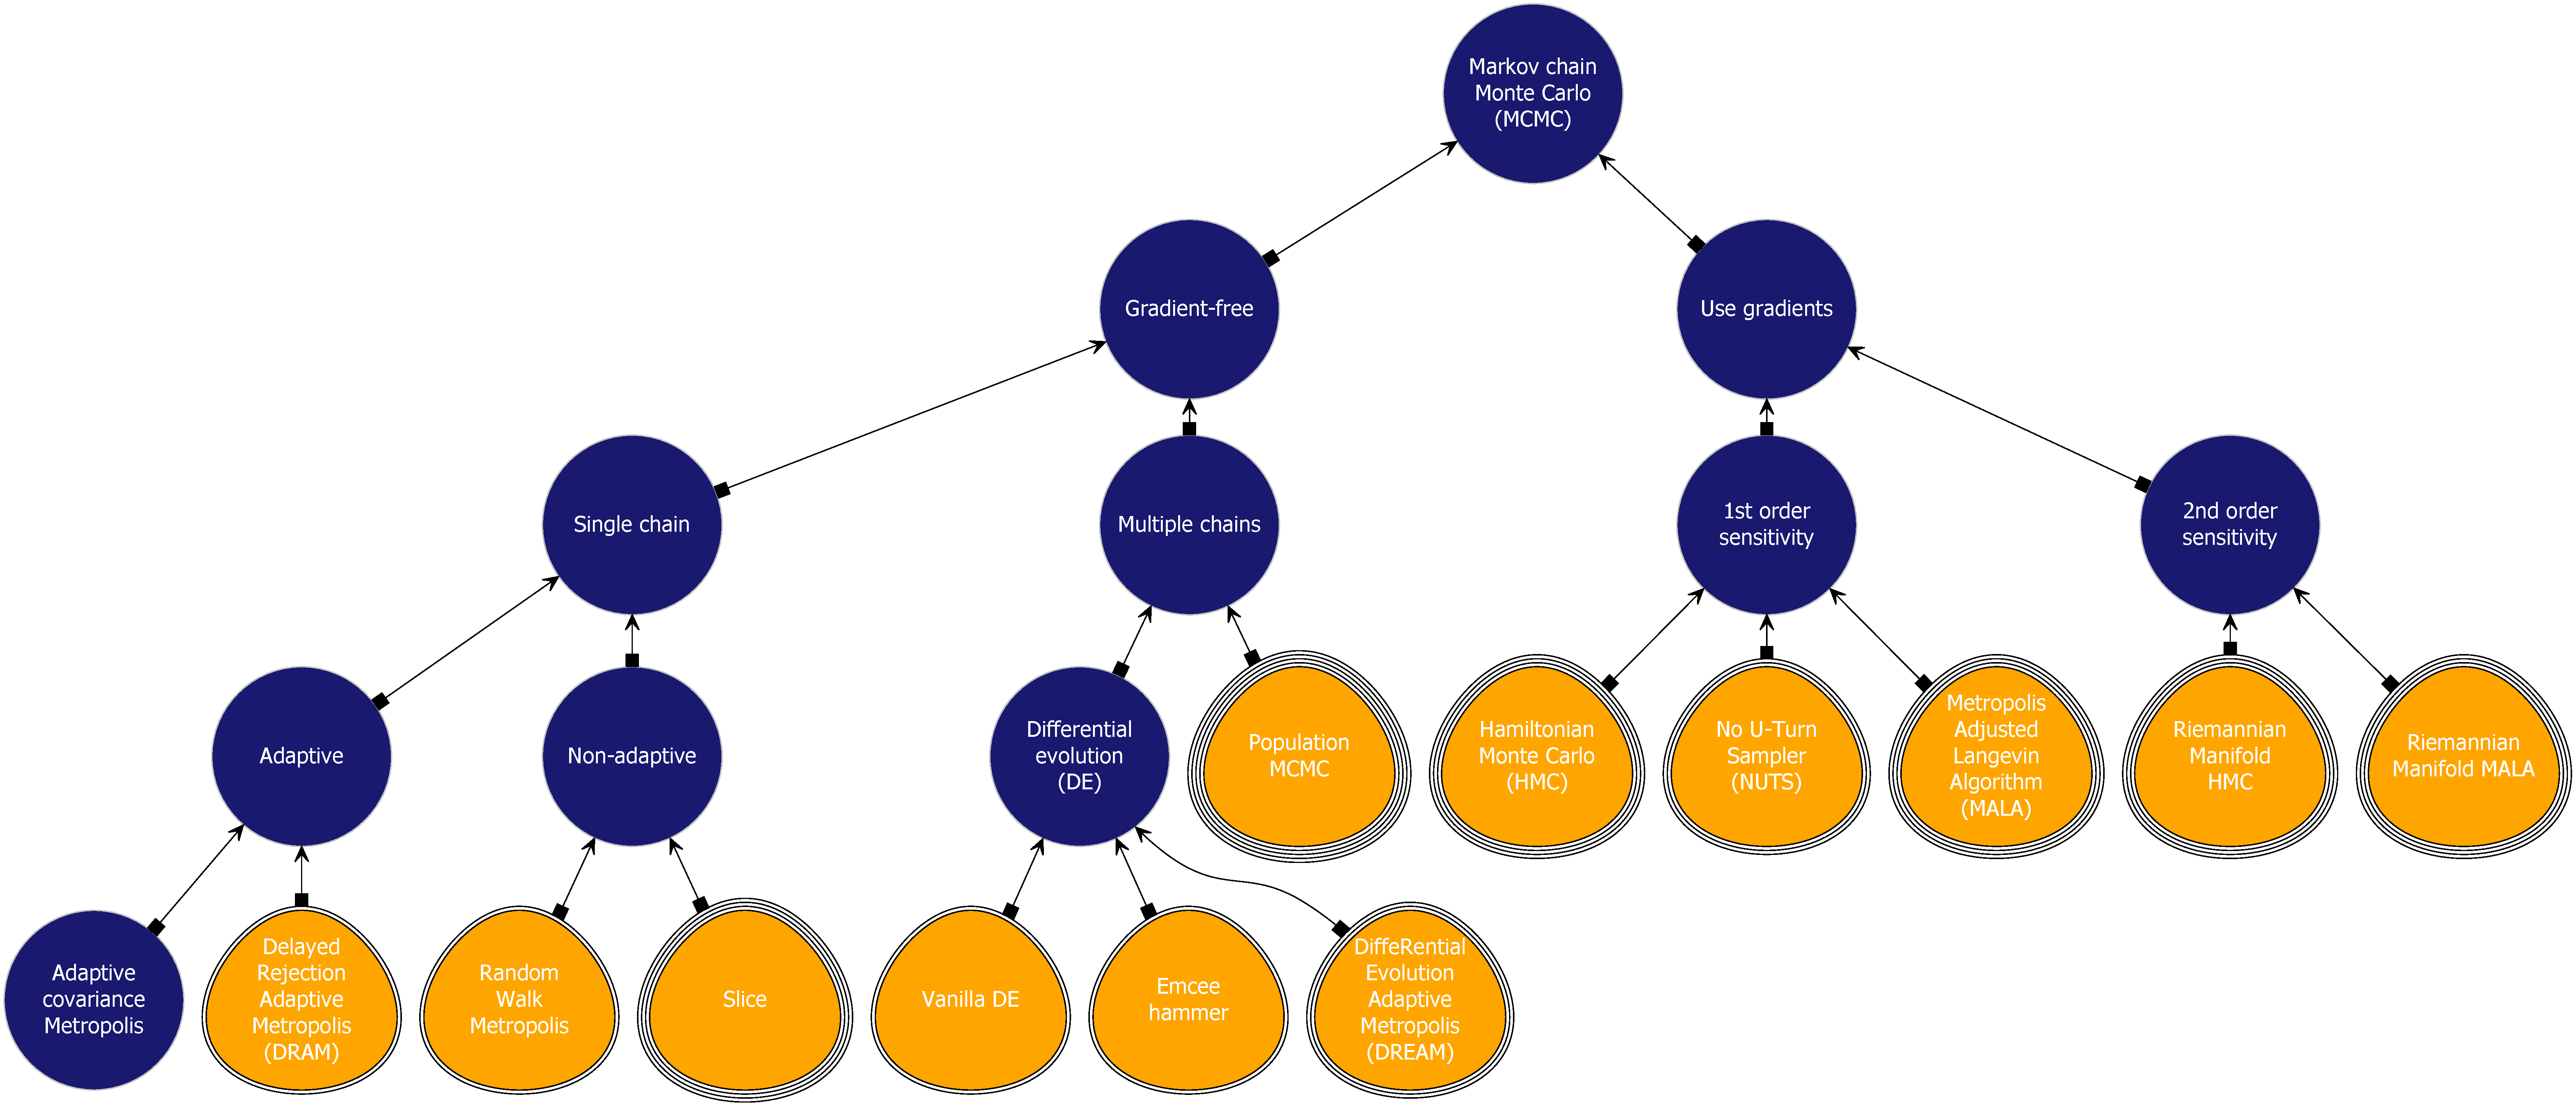
\includegraphics[width=1\textwidth]{./Figures/hierarchy-samplers-mcmc.pdf}}
	\end{figure}
	
\end{frame}

\begin{frame}
	\frametitle{PINTS: optimisers}
	
	Optimisation more ``solved'' than sampling and have two families in PINTS:
	
	\begin{itemize}
		\item Gradient-free: CMAES, XNES, SNES, Nelder-mead, PSO, SHGO (planned);
		\item 1st order sensitivities: gradient descent, L-BFGS (planned).
	\end{itemize}
	
\end{frame}


\begin{frame}
\frametitle{Conclusions}

\begin{itemize}
	\item Inference for ODE models is generally hard;
	\item Stan and PINTS are your current best bet for inference.
\end{itemize}

\end{frame}


\bibliographystyle{authordate1}
\bibliography{Malaria}	 

\end{document}